\chapter{Cơ sở lý thuyết}

\section{Gradient Descent\cite{ref:1}}
Phần lớn các mô hình máy học được xây dựng dựa trên việc tối ưu hóa hàm mất mát hay nói cách khác là tìm cực tiểu của một hàm số biết trước. Đối với các hàm số đơn giản, việc xác đinh các điểm cực tiểu có thể được giải quyết thông qua việc tính toán đạo hàm cấp 1 và cấp 2. Tuy nhiên hàm mất mát của các mô hình máy học hay học sâu thường có số chiều lớn và đạo hàm phức tạp, do đó khó có thể áp dụng các phương pháp truyền thống để tìm các giá trị cực tiểu. Thay vào đó các mô hình này sử dụng giải thuật Gradient Descent để tìm các điểm cực tiểu của hàm mất mát.

Một hàm số có thể có nhiều điểm cực tiểu địa phương (local minimum) và cực tiểu toàn cục (global minimum). Ta có thể thấy trên hình \ref{fig:minimums} là đồ thị của một hàm số đơn biến, điểm màu xanh là cực tiểu địa phương, điểm màu đỏ là cực tiểu toàn cục.
\begin{figure}[ht!]
	\centerline{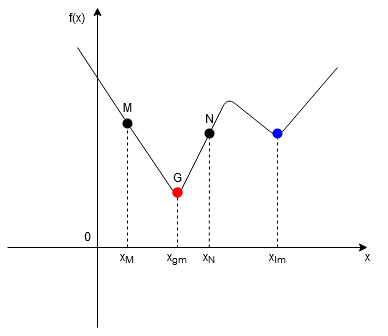
\includegraphics[scale=0.8]{images/minimums.png}}
  	\caption{Cực tiểu địa phương (màu xanh) và cực tiểu toàn cục (màu đỏ)}
  	\label{fig:minimums}
\end{figure}
Giả sử ta có hai điểm $M$ tại $x_M$ và $N$ tại $x_N$ trên đồ thị hình \ref{fig:minimums}, ta gọi điểm cực tiểu toàn cục là $G$. Lúc này ta muốn đưa điểm $M$ và $N$ về xấp xỉ hoặc trùng với vị trí của $G$ bằng giải thuật Gradient Descent. Ta nhận thấy $M$ nằm bên trái $G$ và $f^{'}(x_{M})<0$, nếu $M$ muốn di chuyển về phía $G$ thì $x_{M_{k+1}}=x_{M_{k}}+\delta$ tại bước thứ $k+1$. Ngược lại nếu ta muốn $N$ có $f^{'}(x_{N})>0$ tiến về phía $G$ tại bước tình toán thứ $k+1$ thì $x_{N_{k+1}}=x_{N_{k}}-\delta$. Như vậy để một điểm bất kì $(x,f(x))$ lân cận $G$ trên đồ thị tiến về $G$ thì vị trí của điểm đó phải được cập nhật sau mỗi bước tính toán bằng cách cộng với một lượng $\delta$ với $sign(\delta)=-sign(f^{'}(x))$. Trong thực thế, công thức được sử dụng có dạng:
\begin{equation}
	x_{k+1}=x_{k}-{\mu}f^{'}(x_{k})
\end{equation}
Với $\mu$ là \emph{tốc độ học}, ${\mu}{\in}{\mathbb{R}}$, ${\mu}>0$. Nếu ta chọn $\mu$ lớn thì ta sẽ cần ít số bước tính toán hơn để đến gần vị trí cực tiểu mong muốn nhưng trong nhiều trường hợp độ sai lêch giữa vị trí của điểm tính toán được sau cùng và vị trí của điểm cực tiểu sẽ tương đối cao. Ngược lại, nếu ta chọn $\mu$ nhỏ thì ta sẽ cần nhiều hơn số bước tính toán, bù lại khoảng cách giữa vị trí điểm tính toán được sau cùng và vị trí điểm cực tiểu sẽ có thể rất nhỏ.

Việc áp dụng giả thuật Gradient Descent lên làm đa biến là một sự mở rộng của ví dụ hàm đơn biến ở trên. Cho hàm số $f:{{\mathbb{R}}^n}{\rightarrow}{\mathbb{R}}, n{\in}{\mathbb{N}}^*$, ta cần tìm cực tiểu cho $f(X)$ với $X=\begin{pmatrix}x_0 & ... & x_{n-1}\end{pmatrix}, n{\in}{\mathbb{N}}^*$ từ một điểm khởi đầu $X_0$ bằng giải thuật Gradient Descent. Công thức để tính toán cho mỗi bước là:
\begin{equation}
	X_{k+1}=X_{k}-{\mu}{{\nabla}_X}f\left(X_{k}\right)
\end{equation}
\subsection{Batch Gradient Descent}
Giải thuật Batch Gradient Descent sử dụng tất cả các điểm đầu vào để cập nhật lại vector trọng số tại mỗi bước. Giả sử ta cần tối ưu hàm mất mát của một bài toán hồi quy tuyến tính gồm 30 điểm đầu vào với mỗi điểm gồm 2 tham số $\left(x,f\left(x\right)\right)$ ở hình \ref{fig:batch_gradient_descent}. Để tìm gradient cho mỗi điểm ta cần thực hiện 2 phép toán theo toán tử $\nabla$, đồng thời ta phải tìm gradient cho cả 30 điểm tại mỗi bước lặp và lấy trung bình của các kết quả này để cập nhật trọng số. Tổng số phép toán mà ta phải thực hiện cho tại mỗi bước là $30\times2=60$. Con số này sẽ tăng lên gấp nhiều lần đối với các bài toán thực tế khi số điểm và số tham số là vài triệu hoặc vài tỷ. Nói cách khác thuật toán này không hiệu quả về mặt tính toán với các bài toán máy học với dữ liệu lớn và phải cập nhật liên tục.
\begin{figure}[ht!]
	\centerline{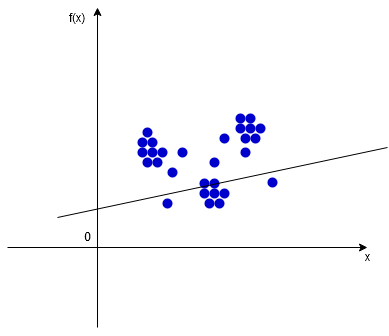
\includegraphics[scale=0.6]{images/batch_gradient_descent.png}}
  	\caption{Batch Gradient Descent với bài toán hồi quy tuyến tính. Toàn bộ số điểm đầu vào đều được dùng để cập nhật các vector trọng số $(a,b)$ cho đường hồi quy tại mỗi bước, với $a$ là độ dốc và $b$ độ sai lệch.}
  	\label{fig:batch_gradient_descent}
\end{figure}
Ngoài ra sau khi đã tìm được nghiêm tối ưu của bài toán. Nếu ta thêm một điểm đầu vào mới vào tập dữ liệu cũ thì việc tính toán phải thực hiện lại từ đầu với toàn bộ điểm đầu vào bao gồm tập điểm đầu vào cũ và điểm mới thêm vào.
\subsection{Stochastic Gradient Descent}
Khác với Batch Gradient Descent giải thuật Stochastic Gradient Descent chỉ dùng gradient của một điểm ngẫu nhiên để cập nhật lại vector trọng số tại mỗi bước. Sau khi đi qua hết tất cả các điểm của tập đầu vào, thứ tự các điểm sẽ được xáo trộn và giải thuật lại tiếp tục với từng điểm. Mỗi một lần giải thuật Stochastic Gradient Descent tính toán xong với một điểm được gọi là một \emph{iteration} còn với toàn bộ tập điểm thì gọi là một \emph{epoch}. Cũng bài toán hồi quy tuyến tính ở trên nhưng với giải thuật Stochastic Gradient Descent (hình \ref{fig:stochastic_gradient_descent}), ta có thể thấy số iteration mà giải thuật Stochastic Gradient Descent phải thực hiện trong một epoch là 30. Số phép tính của một lần tính toán là 2. 
\begin{figure}[ht!]
	\centerline{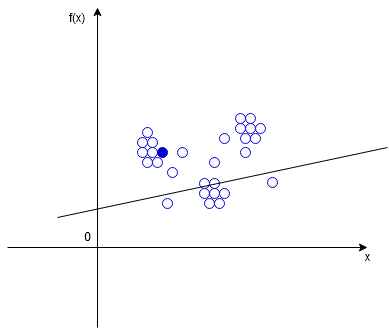
\includegraphics[scale=0.6]{images/stochastic_gradient_descent.png}}
  	\caption{Stochastic Gradient Descent với bài toán hồi quy tuyến tính. Một điểm đầu vào được chọn ngẫu nhiên để cập nhật các vector trọng số $(a,b)$ cho đường hồi quy tại mỗi iteration, với $a$ là độ dốc và $b$ độ sai lệch.}
  	\label{fig:stochastic_gradient_descent}
\end{figure}

Do gradient của 1 điểm chỉ là xấp xỉ gần đúng của trung bình gradient của cả tập điểm nên việc cập nhật tại mỗi iteration sẽ có sai số nhật định, đồng thời các giá trị gradient tính toán được có thể có sư dao động lớn do tập điểm đầu vào thường bị tác động bởi nhiễu. Trên thực tế thì kết quả của giải thuật này có mức độ tối ưu khá tốt và hiệu quả tính toán cao. Sau khi đã hoàn thành tính toán trên tập dữ liệu cũ, nếu như có những điểm mới được thêm vào thì ta chỉ cần chạy giải thuật với các điểm mới mà không cần phải chạy lại giải thuật với toàn bộ các điểm như Batch Gradient Descent.
\subsection{Mini-batch Gradient Descent}
Mini-batch Gradient Descent là sự kết hợp của Batch Gradient Descent và Stochastic Gradient Descent. Một mini-batch sẽ có $n$ điểm với $1<n{\leq}N$, $N$ là tống số điểm của tập dữ liệu đầu vào. Việc chia tập điểm ban đầu thành các batch sẽ được thực hiện một cách ngẫu nhiên. Mỗi một lần giải thuật xử lý xong một  batch sẽ là một iteration và sau khi tất cả các batch được xử lý thì sẽ là một epoch. Như vậy $no\_batch=\frac{N}{n}$. Phương pháp này cho kết quả gần với Batch Gradient Descent nhưng không dùng nhiều tài nguyên tính toán như Batch Gradient Descent và không cần phải lặp lại nhiều lần như Stochastic Gradient Descent.
\begin{figure}[ht!]
	\centerline{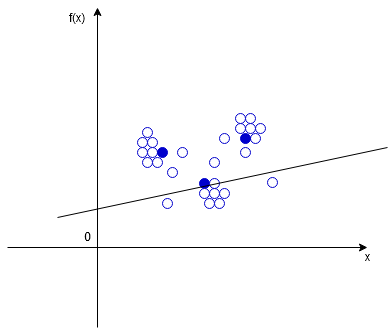
\includegraphics[scale=0.6]{images/mini_batch_gradient_descent.png}}
  	\caption{Mini-batch Gradient Descent với bài toán hồi quy tuyến tính. Một batch sẽ gồm ba điểm đầu vào được chọn ngẫu nhiên để cập nhật các vector trọng số $(a,b)$ cho đường hồi quy tại mỗi iteration, với $a$ là độ dốc và $b$ độ sai lệch. Một epoch sẽ gồm mười batch.}
  	\label{fig:mini_batch_gradient_descent}
\end{figure}
\subsection{Điều kiện dừng của giải thuật}
Ta đã biết các giải thuật Gradient Descent sẽ cần phải thực hiện rất nhiều vòng lặp tính toán để có thể hội tụ. Tuy nhiên rất khó để nói được khi nào có thể dừng được giải thuật. Trong thực tế có nhiều cách khác nhau được dùng để chọn số bước tính toán:
\begin{enumerate}
	\item Chọn một số lương vòng lặp nhất định dựa vào một số tiêu chí như số lượng dữ liệu đầu vào. Cách làm này có thể cho kết quả không đủ tốt, có thể nghiệm tối ưu nằm ở các bước trước hoặc sau điểm kết thúc.
	\item Kiểm tra sự thay đổi của hàm mất mát giữa hai lần cập nhật liên tiếp, nếu sự sai lêch đạt tới ngưỡng đủ nhỏ thì ngưng giải thuật. Tuy nhiên nếu trên đồ thị của hàm mất mát có một vùng bằng phẳng nhưng không phải là cực tiểu thì giải thuật sẽ dừng tại điểm này mà không đạt được cực tiểu.
	\item Kiểm tra sự thay đổi của gradient giữa hai lần cập nhật liên tiếp, nếu sự sai lêch đạt tới ngưỡng đủ nhỏ thì ngưng giải thuật. Nhược điểm của phương pháp này là việc tính gradient của các hàm phức tạp khó có thể thực hiện được.
	\item Kiểm tra kết quả của giải thuật để ngừng việc lặp. Việc này cần người thực hiện việc huấn luyên mô hình phải thường xuyên kiểm tra các tham số hiệu năng của giải thuật lên một tập dữ liệu kiểm tra - \emph{validation set} để xem tại thời điểm nào giải thuật có hiệu năng tốt nhất.
\end{enumerate}
\section{Backpropagation\cite{ref:2}}
Xét một mô hình mạng neuron (hình \ref{fig:ann})
\begin{figure}[ht!]
	\centerline{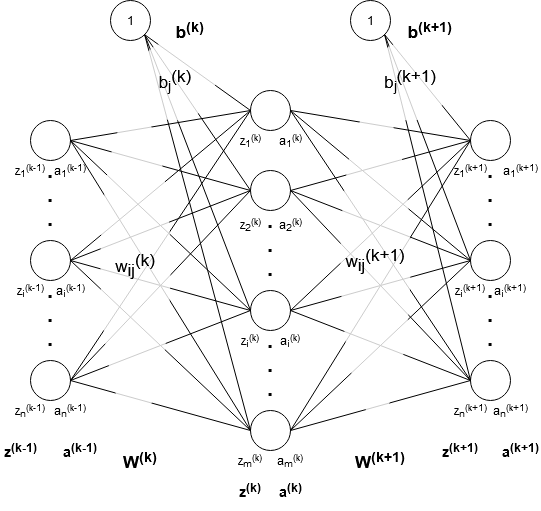
\includegraphics[scale=0.6]{images/ann.png}}
  	\caption{Mô hình mạng neuron đơn giản.}
  	\label{fig:ann}
\end{figure}
Quá trình dữ liệu được đưa vào lớp đầu tiên cho đến khi có kết quả ở lớp sau cùng được gọi là quá trình \emph{feed-forward}.
\begin{align*}
	a^{(0)}&=x \\
	z^{(k)}&={\boldsymbol{W}^{(k)T}}{a^{(k-1)}}+{\boldsymbol{b}}^k,k=1,2,..,N \\
	a^{(l)}&=f^{(k)}\left(z^{(k)}\right),k=1,2,..,N \\
	\widehat{y}&=a^{(N)}
\end{align*}
Ta thấy với mô hình này, hàm mất mát $J\left({\boldsymbol{W}},{\boldsymbol{b}},{\boldsymbol{X}},{\boldsymbol{Y}}\right)$ sẽ phụ thuộc vào tập các ma trận trọng số $\boldsymbol{W}$ và tập các vector bias của mỗi lớp $\boldsymbol{b}$. Việc tính gradient của làm mất mát phụ thuộc vào việc tính các đạo hàm riêng ${\frac{{\partial}J}{{{\partial}\boldsymbol{W}}^{(k)}}}$; ${\frac{{\partial}J}{{\partial}\boldsymbol{b}^{(k)}}}$, ${\forall}k=1,2,..,N$. Đối với bài toán hồi quy tuyến tính thì hàm mất mát là hàm trung bình bình phương sai số (Mean Square Error - MSE), lúc này
\begin{equation}
	J
	\left(
		{\boldsymbol{W}},{\boldsymbol{b}},{\boldsymbol{X}},{\boldsymbol{Y}}
	\right)
	=
	{
		{\frac{1}{M}} 
		{\sum_{i=1}^{(M)}} 
		{ { {\parallel} y_i - \widehat{y_i} {\parallel} }_2 }^2
	}
	=
	{
		{\frac{1}{M}} 
		{\sum_{i=1}^{(M)}} 
		{ { {\parallel} y_i - {a_i}^{(N)} {\parallel} }_2 }^2
	}
\end{equation}
Với $N$ là số điểm trong tập điểm đầu vào. Ta nhận thấy để tìm các đạo hàm riêng của $J$ với ${\boldsymbol{W}}$ và ${\boldsymbol{b}}$ trong trường hợp này là rất khó vì phương trình của $J$ không phụ thuộc trực tiếp vào ${\boldsymbol{W}}$ và ${\boldsymbol{b}}$. Để có thể hiện thực các giải thuật thuộc họ Gradient Descent thì phương pháp thường được sử dụng là Backpropagation. Phương pháp này sẽ cập nhật các trọng số theo chiều từ layer cuối cùng đến layer đầu tiên. Đầu tiên giải thuật sẽ tính đạo hàm của hàm mất mát theo ma trận trọng số của lớp cuối cùng.
\begin{align*}
	\frac
		{ {\partial} J }
		{ {\partial} {w_{ij}^{(N)}} }
	&=
	\frac
		{ {\partial} J }
		{ {\partial} {z_{j}^{(N)}} }
	{\cdot}
	\frac
		{ {\partial} {z_{j}^{(N)}} }
		{ {\partial} {w_{ij}^{(N)}} } \\
	&=
	{e_{j}^{(N)}}
	{
		\frac
			{ {\partial} \left(
							{w_{ij}^{(N)T}}
							a^{(N-1)}
							+
							{b_{j}^{(N)}}
						 \right)
			}
			{ {\partial} {w_{ij}^{(N)}} }
	}\\
	&={e_{j}^{(N)}}{a_{i}^{(N-1)}}
\end{align*}
Với ${e_{j}^{(N)}}=\frac{{\partial}J}{{\partial}{z_{j}^{(N)}}}$ có thể tính được tương đối dễ dàng. Tương tự ta có đạo hàm riêng của $J$ với bias ở lớp cuối cùng.
\begin{align*}
	\frac
		{ {\partial} J }
		{ {\partial} {b_{j}^{(N)}} }
	&=
	\frac
		{ {\partial} J }
		{ {\partial} {z_{j}^{(N)}} }
	{\cdot}
	\frac
		{ {\partial} {z_{j}^{(N)}} }
		{ {\partial} {b_{j}^{(N)}} } \\
	&={e_{j}^{(N)}}
\end{align*}
Các công thức trên cũng đúng với một lớp bất kỳ trong mạng neuron. Ta lấy mô hình hai lớp liên tiếp của một mạng neuron ở hình \ref{fig:ann} để đưa ra công thức tổng quát như sau:
\begin{align*}
	\frac
		{ {\partial} J }
		{ {\partial} {w_{ij}^{(k)}} }
	&=
	\frac
		{ {\partial} J }
		{ {\partial} {z_{j}^{(k)}} }
	{\cdot}
	\frac
		{ {\partial} {z_{j}^{(k)}} }
		{ {\partial} {w_{ij}^{(k)}} } \\
	&=
	{e_{j}^{(k)}}
	\frac
		{ {\partial} \left(
						{w_{ij}^{(k)T}}
						a^{(k-1)}
						+
						{b_{j}^{(k)}}
					 \right)
		}
		{ {\partial} {w_{ij}^{(N)}} } \\
	&={e_{j}^{(k)}}{a_{i}^{(k-1)}} \\ \\
	\frac
		{ {\partial} J }
		{ {\partial} {b_{j}^{(k)}} }
	&=
	\frac
		{ {\partial} J }
		{ {\partial} {z_{j}^{(k)}} }
	{\cdot}
	\frac
		{ {\partial} {z_{j}^{(k)}} }
		{ {\partial} {b_{j}^{(k)}} } \\
	&={e_{j}^{(k)}}
\end{align*}
Ta sẽ tính $e_{j}^{(k)}$ như sau:
\begin{align*}
	{e_{j}^{(k)}}
	&=
	{\frac
		{ {\partial} J }
		{ {\partial} {z_{j}^{(k)}} }
	}
	=
	{\frac
		{ {\partial} J }
		{ {\partial} {a_{j}^{(k)}} }
	}
	{\cdot}
	{\frac
		{ {\partial} {a_{j}^{(k)}} }
		{ {\partial} {z_{j}^{(k)}} }
	} \\
	&=\left( 
			 {\sum_{l=1}^{d^{(k+1)}}} 
			 {\frac
			 	{ {\partial} J }
			 	{ {\partial} {z_{l}^{k+1}} } 
			 }
			 {\cdot}
			 {\frac
			 	{ {\partial} {z_{l}^{(k+1)}} }
			 	{ {\partial} {a_{j}^{(k)}} } 
			 }
		\right) 
		{
			{f^{(k)'}} \left( 
					{z_{j}^{(k)}} 
				 \right)
		} \\
	&=\left( 
			 {\sum_{l=1}^{d^{(k+1)}}} 
			 e_{l}^{(k+1)}
			 {\cdot}
			 w_{jl}^{(k+1)}
		\right) 
		{
			{f^{(k)'}} \left( 
					{z_{j}^{(k)}} 
				 \right)
		}
\end{align*}
Ta có $f:{\mathbb{R}}{\rightarrow}[0,1]$ là hàm kích (activation function) hay còn gọi là hàm bao tại một node trong mạng neuron, $a_{j}^{k}=f\left(z_{j}^{k}\right)$, do dó ta có đạo hàm riêng của $a_{j}^{k}$ theo $z_{j}^{k}$ chính là đạo hàm của $f$. Ngoài ra do $a_{j}^{k}$ trực tiếp tham gia vào việc tính các $z_{l}^{k+1},l=1,2,..,d^{(k+1)}$ nên ${\frac{{\partial}J}{{\partial}{a_{j}^{k}}}}$ có thể tách ra thành tổng của tích các đạo hàm riêng như dòng thứ hai. Tương tự như vậy ta có thể tính
\begin{equation}
	\frac
		{ {\partial} J }
		{ {\partial} {b_{j}^{(k)}} }
	= {e_{j}^{(k)}}
\end{equation}
Việc tính ${e_{j}^{k}}$ sẽ phụ thuộc vào kết quả của ${e_{j}^{k+1}}$ do đó phương pháp này được gọi là Backpropagation.
Các bước để thực hiện giải thuật Backpropagation cho một mạng neuron nhân tạo gồm:
\begin{enumerate}
	\item Feedforward: Với mỗi giá trị đầu vào của x, tính giá trị đầu ra của mạng neuron, đồng thời lưu lại các kết quả ${\boldsymbol{a}}^{(k)}$ tại mỗi lớp.
	\item Với mỗi node thứ $j$ ở lớp ngoài cùng tính
\begin{equation}
	{e_{j}^{(N)}}
	=
	\frac
		{ {\partial} J }
		{ {\partial} {z_{j}^{(N)}} }
\end{equation}
	\item Từ đó suy ra:
\begin{align*}
	\frac
		{ {\partial} J }
		{ {\partial} {w_{ij}^{(N)}} }
	&=
	{a_{i}^{(N-1)}}
	{e_{j}^{(N)}} \\
	\frac
		{ {\partial} J }
		{ {\partial} {b_{j}^{(N)}} }
	&=
	{ e_{j}^{(N)} }
\end{align*}
	\item Với $k=N-1,N-2,...,1$ tìm $e_{j}^{(k)}$
\begin{equation}
	e_{j}^{(k)}
	=
	\left( 
		{\sum_{l=1}^{d^{(k+1)}}}
		e_{l}^{(k+1)}
		{\cdot}
		w_{jl}^{(k+1)}
	\right) 
	{
		{f^{(k)'}} 
		\left( 
			{z_{j}^{(k)}} 
	 	\right)
	}
\end{equation}
	\item Cập nhật đạo hàm cho từng trọng số và bias:
\begin{align*}
	\frac
		{ {\partial} J }
		{ {\partial} {w_{ij}^{(k)}} }
	&=
	{a_{i}^{(k-1)}}
	{e_{j}^{(k)}} \\
	\frac
	{ {\partial} J }
		{ {\partial} {b_{j}^{(k)}} }
	&=
	{ e_{j}^{(k)} }
\end{align*}
\end{enumerate}
\section{Mạng neuron tích chập\cite{ref:3}\cite{ref:4}}
Mạng neuron tích chập (tiếng Anh: Convolutional Neural Network - CNN) là một loại mạng neuron dùng riêng cho các bài toán về hình ảnh. Bên trong mạng neuron tích chập vẫn là các neuron có các trọng số và bias có thể cập nhật được để học các đặc trưng của hình ảnh.

Các lớp của mạng neuron tích chập được bố trí theo ba chiều: chiều rộng (tiếng Anh: width), chiều cao (tiếng Anh: height), chiều sâu (tiếng Anh: depth). Chiều sâu ở đây muốn nói tời chiều sâu của miền các neuron kích hoạt (tiếng Anh: activation volume) chứ không phải là chiều sâu của cả mạng neuron. Các neuron ở lớp sau sẽ chỉ được kết nối với một phần nhỏ các neuron ở lớp trước chứ không phải là toàn bộ như trong các mạng neuron thông thường. Ta lấy ví dụ mạng CIFAR-10 (hình \ref{fig:cnn}), miền các neuron kích hoạt ở mạng neuron này có kích thước các chiều là $32{\times}32{\times}3$ (\emph{rộng} ${\times}$ \emph{cao} ${\times}$ \emph{sâu}). Lớp cuối cùng của CIFAR-10 sẽ có kích thước các chiều là $1{\times}10{\times}10$ ứng với vector điểm cho các nhãn cần được phân loại (tiếng Anh: class scores).
\begin{figure}[ht!]
	\centerline{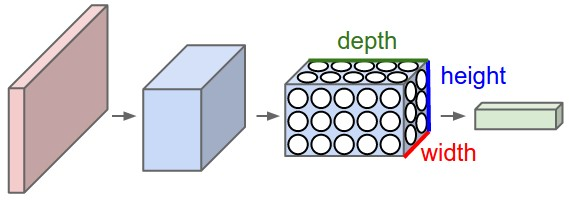
\includegraphics[scale=0.6]{images/cnn.jpeg}}
  	\caption{Mô hình mạng neuron tích chập đơn giản. Lớp nhận hình ảnh vào màu đỏ là một lớp có cấu trúc ba chiều với chiều rộng và chiều cao là chiều rộng và chiều cao của hình ảnh đầu vào, chiều sâu bằng ba ứng với ba kênh màu đỏ, xanh lá và xanh dương. Các lớp của mạng neuron tích chập sẽ chuyển đổi một nhóm các ma trận thành một nhóm các ma trận khác. Lớp ngoài cùng là lớp phân loại, có kích thước các chiều tương ứng với một vector.}
  	\label{fig:cnn}
\end{figure}
Một mạng neuron tích chập thông thường sẽ được cấu tạo từ ba loại lớp neuron: lớp tích chập (tiếng Anh: convolutional layer), lớp pooling (tiếng Anh: pooling layer) và lớp đầy đủ kết nối (tiếng Anh: fully-connected layer).
\subsection{Lớp tích chập}
Trong lớp này đầu vào lớp đầu tiên sẽ là một ảnh màu có ba kênh màu: đỏ, xanh lá, xanh dương (hình \ref{fig:image_convol_0}). Đầu ra của các lớp trước sẽ là đầu vào của các lớp sau. Các tensor trong mạng tích chập được gọi là các tensor.
\begin{figure}[ht!]
	\centerline{
\includegraphics[scale=0.2]{images/image_convol_0.png}}
  	\caption{Hình ảnh đầu vào gồm ba kênh màu được mô hình hóa thành tensor với chiều cao và chiều rộng là chiều cao và chiều rộng của ảnh, chiều sâu là ba.}
  	\label{fig:image_convol_0}
\end{figure}
Sau đó một bộ lọc có kích thước $m \times n \times 3$ (tiếng Anh: kernel) sẽ được trượt qua tensor của ảnh đầu vào. Ở mỗi kênh màu, lớp tương ứng của kernel sẽ hoạt động như một cửa sổ trượt (tiếng Anh: sliding window).
\begin{figure}[ht!]
	\centerline{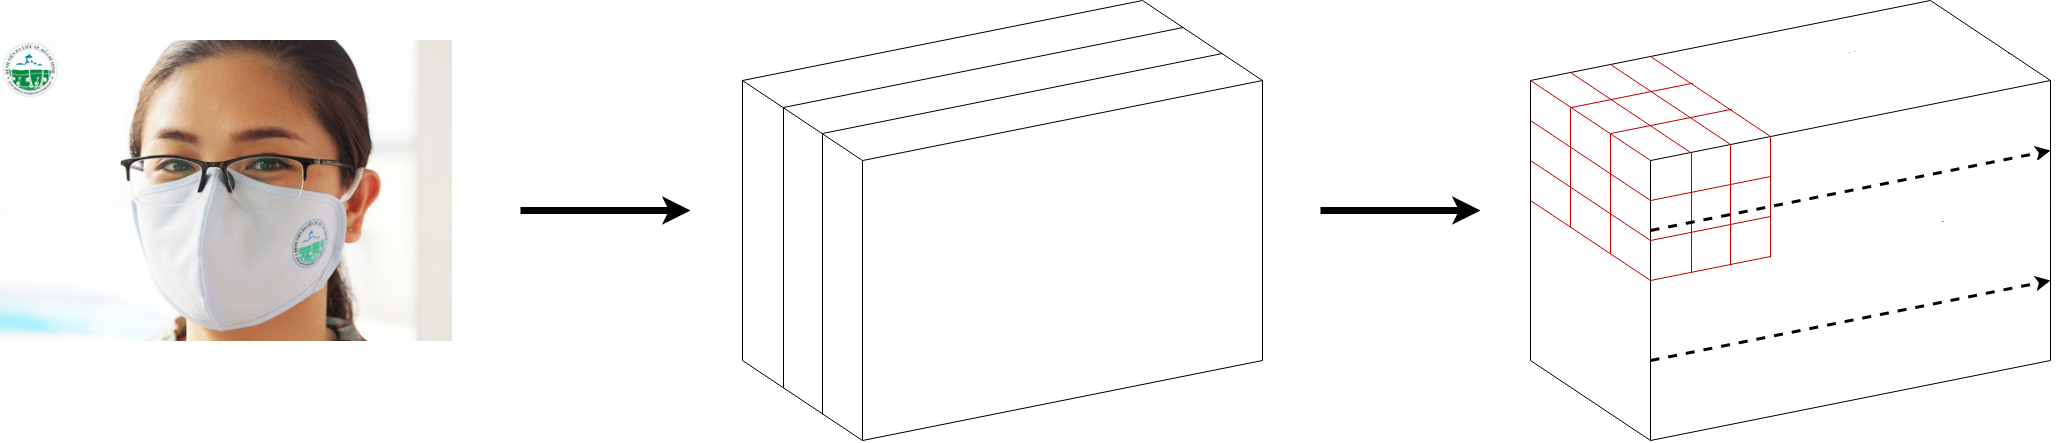
\includegraphics[scale=0.2]{images/image_convol_1.png}}
  	\caption{Hình ảnh sau khi được đưa qua đầu vào và chuyển đổi thành dữ liệu ba chiều sẽ được đưa vào lớp convolution đầu tiên. Một kernel có kích thước $3 \times 3 \times 3$ (góc trên bên trái của mô hình ngoài cùng bên phải) được trượt qua hình đầu vào.}
  	\label{fig:image_convol_1}
\end{figure}
Nhắc lại một chút về phép toán của cửa sổ trượt trên ảnh trắng đen. Giả sử ta có một cửa sổ trượt có kích thước $3 \times 3$ đang quét qua một hình trắng đen (hình \ref{fig:sliding_window}), tại vị trí như trên hình việc tính toán giá trị đầu ra được thực hiện như sau
\begin{equation}
	1 \times 0 + 1 \times 0 + 1 \times 0 + 6 \times 1 + 7 \times 1 + 9 \times 1 + 1 \times 0 + 0 \times 0 + 0 \times 0 = 22 
\end{equation}
\begin{figure}[ht!]
	\centerline{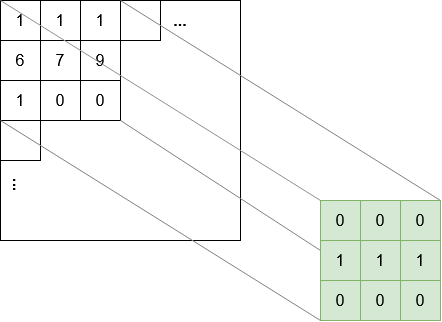
\includegraphics[scale=0.6]{images/sliding_window.png}}
  	\caption{Ví dụ về phép toán cửa sổ trượt với kích thước $3 \times 3$.}
  	\label{fig:sliding_window}
\end{figure}
Ngoài ra, ta còn hai khái niệm cần nhắc tới là stride và padding. 
\begin{itemize}
	\item Với stride bằng một thì cửa sổ trượt sẽ di chuyển tuần tự qua tất cả các ô của ma trận. Tổng quát với $stride = k$ thì các điểm ảnh được cửa sổ trượt đi qua của một ma trận có kích thước $m {\times} n$ sẽ là $x_{1+i {\times} k,1+j {\times} k}$ với $i,j \in \mathbb{N}; 1+i \times k \leq m; 1+j \times k \leq n$.
	\item Đối với các điểm ảnh ở gần biên, nếu như trong vùng cửa sổ không có những chỗ không tồn tại giá trị điểm ảnh thì các phương pháp chèn giá trị (tiếng Anh: padding) sẽ được sử dụng để thay làm các giá trị tính toán. Một trong các cách padding phổ biến là dùng các giá trị bằng không (tiếng Anh: zero padding).
\begin{figure}[ht!]
	\centerline{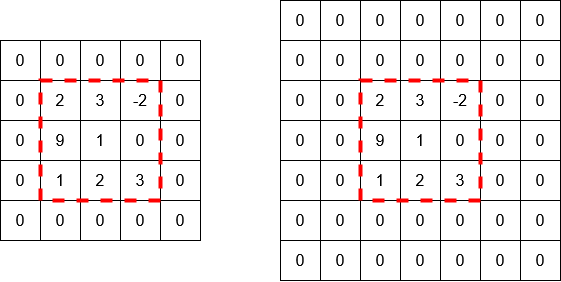
\includegraphics[scale=0.6]{images/padding.png}}
  	\caption{Bên trái, ma trận $3 \times 3$ được zero padding với $padding=1$. Bên phải, ma trận $3 \times 3$ được zero padding với $padding=2$}
  	\label{fig:padding}
\end{figure}
\end{itemize}
Như vậy, nếu đầu vào của phép tính tích chập là ma trận $X$ có kích thước $m \times n$ với cửa sổ trượt có kích thước $k \times k, stride=s, padding=p$ thì đầu ra sẽ là một ma trận $Y$ có kích thước 
$\left( 
	\frac
		{{m-k+2p}}
		{8}
	+1
\right)
\times
\left( 
	\frac
		{{n-k+2p}}
		{8}
	+1
\right)$

Việc tính toán tại mỗi kênh màu của hình khi kernel đi qua cũng gần tương tự với cửa sổ trượt. Kết quả phép toán của ba kênh màu và một bias sẽ được cộng lại và đưa vào ma trận kết quả. Giả sử ta có một kernel có kích thước $3 \times 3 \times 3$ như hình \ref{fig:kernel}.
\begin{figure}[ht!]
	\centerline{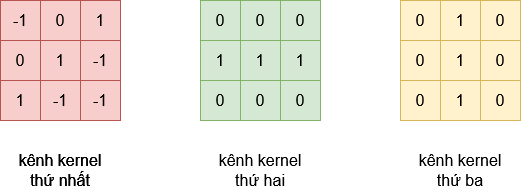
\includegraphics[scale=0.6]{images/kernel.png}}
  	\caption{Ví dụ về một kernel có kích thước $3 \times 3 \times 3$.}
  	\label{fig:kernel}
\end{figure}
Dữ liệu một ảnh đầu vào gồm ba kênh màu, khi đi qua lớp tích chập đầu tiên sẽ được tính toán như hình \ref{fig:kernel_calculation}
\begin{figure}[ht!]
	\centerline{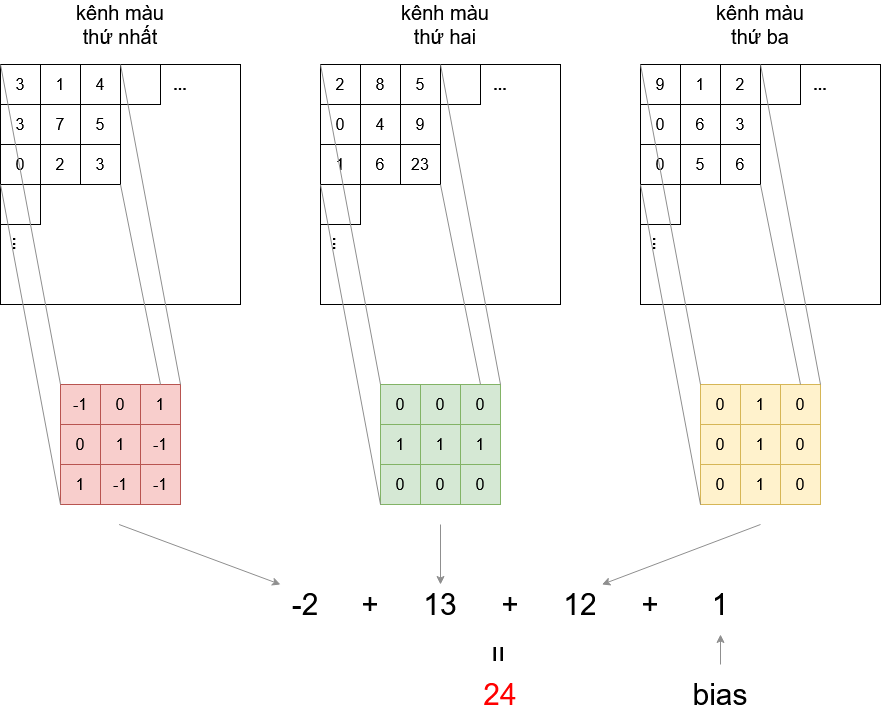
\includegraphics[scale=0.4]{images/kernel_calculation.png}}
  	\caption{Ví dụ về phép toán của một kernel lên một vị trí của ảnh trong lớp tích chập.}
  	\label{fig:kernel_calculation}
\end{figure}
Sau khi kernel đã quét qua hết các điểm ảnh mong muốn thì kết quả nhận được sẽ là một ma trận. Mỗi một kernel khác nhau sẽ trích xuất ra được một đặc trưng khác nhau của ảnh. Do đó một lớp tích chập sẽ có nhiều kernel để lấy các đặc trưng khác nhau. Lúc này đầu ra sẽ là một tensor gồm nhiều ma trận. Nếu như có $k$ kernel được dùng tại một lớp tích chập thì đầu ra sẽ có chiều sâu bằng $k$, chiều rộng và chiều cao sẽ bằng chiều rộng và chiều cao của ảnh đầu vào. Đầu ra của lớp tích chập trước sẽ là đầu vào của lớp tích chập sau.
\begin{figure}[ht!]
	\centerline{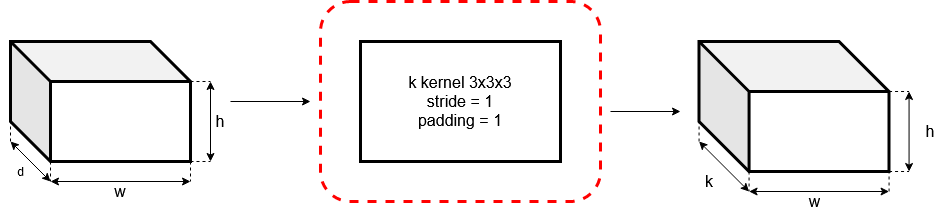
\includegraphics[scale=0.4]{images/convol_layer_in_out.png}}
  	\caption{Một lớp tích chập có $k$ kernel với kích thước $3 \times 3 \times 3$, $stride = 1$, $padding = 1$. Đầu vào là một tensor có kích thước $h \times w \times d$ đầu ra của phép tích chập lên tensor này khi khối tích chập có các thông số ở trên là một tensor có kích thước $h \times w \times k$}
  	\label{fig:convol_layer_in_out}
\end{figure}
Tổng quát hóa, với một lớp tích chập với $K$ kernel có kích thước $N \times N \times D$ (với D là chiều sâu của đầu vào và là số lẻ), $stride=S$, $padding=P$. Đầu vào là một tensor có kích thước $H \times W \times D$ thì kích thước của tensor đầu ra sẽ là
$\left( 
	\frac
		{{H-F+2P}}
		{S}
	+1
\right)
\times
\left( 
	\frac
		{{W-F+2P}}
		{S}
	+1
\right)
\times
K$

Đầu ra của lớp tích chập sẽ đi qua hàm kích hoạt trước khi được đưa vào lớp tích chập tiệp theo. Mỗi kernel với kích thước $N \times N \times D$ sẽ có một hệ số bias tương ứng với tổng số các tham số của môt kernel là $N \times N \times D+1$, với $K$ kernel thì số tham số sẽ là $K \times (N \times N \times D+1)$.
\subsection{Lớp pooling}
Việc tính toán với toàn bộ dữ liệu đầu vào của ảnh có độ phân giải lớn và kích thước lớn trên mạng neuron tích chập thường không hiệu quả về mặt tính toán do sẽ có nhiều điểm ảnh miêu tả cùng một đặc trưng. Do đó lớp pooling được dùng ở giữa các lớp tích chập để giảm kích thước của các tensor nhưng vẫn không làm mất đi các đặc trưng của dữ liệu.

Cho một lớp pooling có kích thước cửa sổ trượt là $N \times N$, đầu vào là một tensor có kích thước $H \times W \times D$. Ta chia tensor này thành $D$ ma trận $H \times W$. Với mỗi ma trận ta lần lượt trượt cửa sổ trượt của lớp pooling lên tưng điểm ảnh. Trong vùng dữ liệu của cửa sổ trượt ta sẽ tìm giá trị lớn nhất hoặc trung bình của các giá trị để đưa vào ma trận mới.
\begin{figure}[ht!]
	\centerline{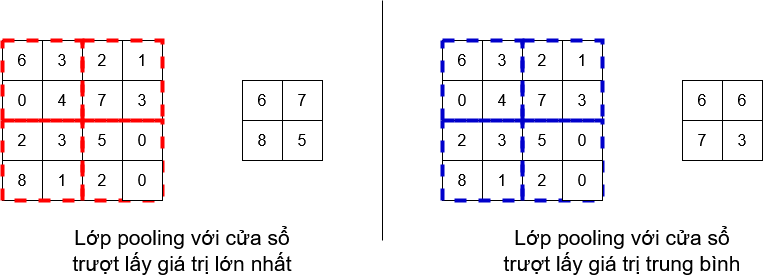
\includegraphics[scale=0.4]{images/pooling.png}}
  	\caption{Bên trái, lớp pooling với cửa sổ trượt lấy giá trị lớn nhất với kích thước cửa sổ $2 \times 2, stride=1, padding=0$. Bên phải, lớp pooling với cửa sổ trượt lấy giá trị trung bình với kích thước cửa sổ $2 \times 2, stride=2, padding=0$.}
  	\label{fig:pooling}
\end{figure}
Một số mô hình mạng neuron tích chập sẽ dùng $stride>1$ trong lớp tích chập để làm giảm kích thước dữ liệu thay vì dùng lớp pooling. Ngoài ra, trong thực tế lớp pooling thường được sử dụng với kích thước cửa sổ trượt $2 \times 2, stride=2, padding=0$. Chiều cao và chiều rộng của tensor đầu ra sẽ giảm đi một nửa còn chiều sâu vẫn giữ nguyện.
\subsection{Lớp đầy đủ kết nối}
Hình ảnh sau khi qua các lớp tích chập và pooling thì đầu ra sẽ là một tensor chứa các đặc trưng mà mô hình trích xuất được. Tensor có kích thước $H \times W \times D$ tại lớp tích chập cuối cùng sẽ được chuyển thành một vector có chiều dài $H \times W \times D$. Sau đó vector này sẽ được đưa vào các lớp đầy đủ kết nối để đưa ra kết quả dự đoán cho ảnh.
\subsection{Mô hình mạng neuron tích chập}
Ảnh đầu vào $\rightarrow$ [Lớp tích chập $\rightarrow$ Lớp pooling] $\times n \rightarrow$ [Lớp liên kết hoàn toàn] $\times m \rightarrow$ Đầu ra, với $m,n \in {\mathbb{N}}^*$.
\begin{figure}[ht!]
	\centerline{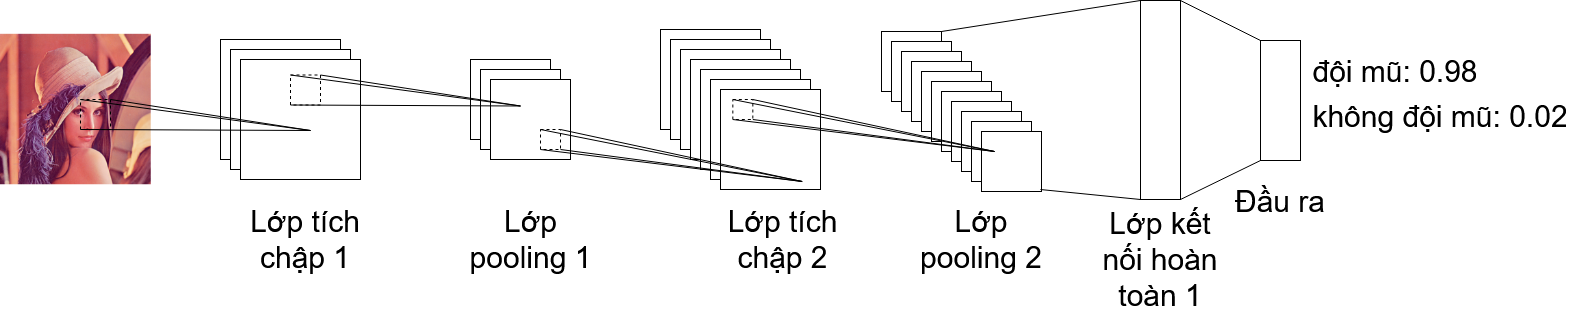
\includegraphics[scale=0.25]{images/cnn_simplified.png}}
  	\caption{Mạng neuron tích chập gồm hai lớp tích chập và pooling, một lớp kết nối đầy đủ.}
  	\label{fig:cnn_simplified}
\end{figure}
\section{YOLOv3\cite{YOLOv3-1}\cite{ref:6}}
YOLO - You Only Look Once là một trong những mô hình nhận diện thời gian thực hiện đại nhất và đang được sử dụng cho nhiều bài toán nhận diện, theo dõi khác nhau. Không như những mạng CNN hay R-CNN  trước đây, thay vì sử dung phương pháp dự đoán trên từng miền (tiếng Anh: region proposal method) và cửa sổ trượt (tiếng Anh: sliding window) để phát hiện vật thể trong từng vùng nhỏ trong khung hình và tiến hành phân loại vật thể đó. YOLO sử dụng cả khung hình để nhận diện vật thể, các đặc trưng của vùng nền phía sau (tiếng Anh: background) cũng được dùng trong quá trình huấn luyện. Do vậy YOLO có thể nhận diện vật thể một cách nhanh chóng trong một khung hình với độ chính khác cao chỉ với một lần xử lý, đó cũng là lý do vì sao mô hình này được gọi là Bạn Chỉ Cần Nhìn Một Lần (tiếng Anh: You Only Look Once).
\subsection{Unified Detection}
Hình ảnh đầu vào được chia thành một mạng lưới ô vuông (tiếng Anh: grid cell) có kích thước $S \times S$. Nếu như tâm của một vật thể nằm ở tâm của của một ô thì ô đó sẽ chịu trách nhiệm trong việc nhận diện vật thể đó.
\begin{figure}[ht!]
	\centerline{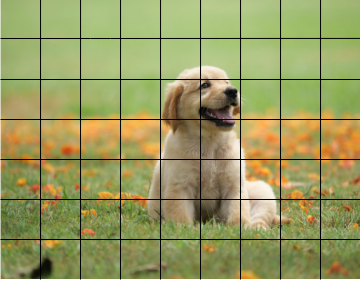
\includegraphics[scale=0.6]{images/grid_cell.png}}
  	\caption{Hình ảnh được chia thành mạng lưới ô vuông $S \times S$.}
  	\label{fig:grid_cell}
\end{figure}
Mỗi ô sẽ dự đoán $B$ bounding box và độ tin cậy (tiếng Anh: confidence score) của từng bounding box. Gọi $Pr(Object)$ là xác xuất của vật thể nằm trong một ô với $Pr(Object) \in \mathbb{R}, 0 \leq Pr(Object) \leq 1$. $IOU$ - intersection over union là tỷ lệ giữa diện tích miền giao và diện tích miền hợp của bounding box dự đoán được và bounding box được tạo sẵn để huấn luyện (tiếng Anh: ground truth) hình \ref{fig:iou}, $IOU \in \mathbb{R}, 0 \leq IOU \leq 1$.
\begin{figure}[ht!]
	\centerline{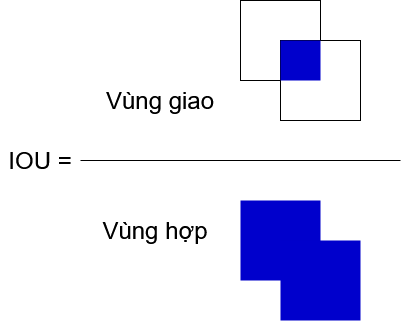
\includegraphics[scale=0.6]{images/iou.png}}
  	\caption{Miêu tả việc tính toán IOU.}
  	\label{fig:iou}
\end{figure}
Độ tin cậy sẽ được định nghĩa bằng $Pr(Object) \times IOU$, nếu như một ô không chứa vật thể thì $Pr(Object)=0$ suy ra độ tin cậy sẽ bằng không, ngược lại nếu một ô chứa vật thể thì $Pr(Object)=1$, lúc này độ tin cậy bằng $IOU$.

Mỗi một bouding box sẽ có năm tham số cần dự đoán: $t_x,t_y,t_w,t_h$ và độ tin cậy. $(t_x,t_y)$ là tọa độ tương đối của tâm bounding box với một ô, nếu gọi offset của một ô trong hình là $(c_x,c_y)$ thì tọa độ của một bounding box so với hình sẽ là $(\sigma \left( t_x \right)+c_x,\sigma \left( t_y \right)+c_y)$. Nếu chiều dài và chiều rộng của bounding box cho trước là $\left( p_w,p_h \right)$ chiều dài và chiều rộng của bounding box được sự đoán sẽ là $\left( p_w \times e^{t_w},p_h \times e^{t_h} \right)$.
\begin{align*}
	b_x &= \sigma \left( t_x \right)+c_x\\
	b_y &= \sigma \left( t_y \right)+c_y\\
	b_w &= p_w \times e^{t_w}\\
	b_h &= p_h \times e^{t_h}
\end{align*}
\begin{figure}[ht!]
	\centerline{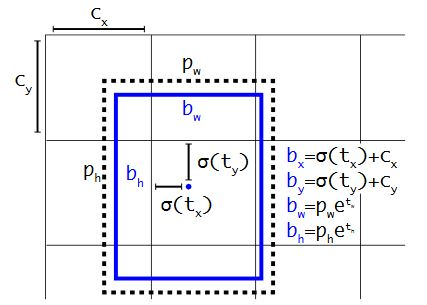
\includegraphics[scale=0.8]{images/bounding_box_prediction.jpg}}
  	\caption{Mô hình dự đoán bounding box của YOLO.}
  	\label{fig:bounding_box_prediction}
\end{figure}
Trong quá trình huấn luyện, hàm mất mát tổng bình phương sai số được sử dụng cho các tọa độ của bounding box. Với một dự đoán $t_*$ có ground truth là ${\widehat{t}}_*$ thì gradient sẽ là hiệu giữa ground truth và kết quả dự đoán được ${\widehat{t}}_* - t_*$.

YOLOv3 sử dụng hàm hồi quy logistic để dự đoán xem một bounding box có chứa vật thể hay không. Nếu như bounding box dự đoán được giao với ground truth nhiều hơn các bounding box trước đó thì kết quả là $1$. Nếu như một bounding box dự đoán được không phải là trường hợp có diện tích giao lớn nhất với ground truth nhưng vẫn có độ tin cậy lớn hơn một ngưỡng xác quyết thì dự đoán với bounding box này sẽ bị bỏ qua. Ngưỡng xác quyết được dùng là $0.5$. Nếu như một bounding box không được đặt vào một ground truth thì sẽ không có các dự đoán về tọa độ và class mà chỉ có dự đoán về sự tồn tại của vật thể.

Độ tin cậy chính là $IOU$ giữa bounding box dự đoán được và bounding box được tạo sẵn. Đối với những ô được dự đoán có vật thể, mô hình sẽ dự đoán thêm $C$ xác suất của các class mà vật thể đó thuộc về $Pr \left( Class_i | Object \right)$ với $Pr \left( Class_i | Object \right) \in \mathbb{R}, 0 \leq Pr \left( Class_i | Object \right) \leq 1, i=1,..,C$. Mỗi ô sẽ chỉ có một tập các giá trị $Pr \left( Class_i | Object \right)$ mà không liên quan tới số lương bounding box $B$.

Khi tiến hành dự đoán, YOLO sẽ nhân các xác suất và độ tin cậy lại với nhau để được xác suất của một class trên một bounding box. 
\begin{equation}
	Pr \left( Class_i | Object \right) \times Pr(Object) \times IOU = Pr \left( Class_i \right) \times IOU
\end{equation}
Hàm mất mát được sử dụng khi huấn luyện để dự đoán các class là hàm binary cross-entropy nhằm giúp mô hình có thể dự đoán đa lớp trong cùng một ô.

Sau cùng ta có hàm mất mát tổng của YOLOv3
\begin{align*}
	Loss =
		&\sum_{i=0}^{S^2} 
		\sum_{j=0}^{B}
		{\mathfrak{1}}^{obj}_{ij}
		\left[
			{
			\left(
				{\widehat{t}}_{x_{ij}}
				-
				t_{x_{ij}}
			\right)
			}^2
			+
			{
			\left(
				{\widehat{t}}_{y_{ij}}
				-
				t_{y_{ij}}
			\right)
			}^2
			+
			{
			\left(
				{\widehat{t}}_{w_{ij}}
				-
				t_{w_{ij}}
			\right)
			}^2
			+
			{
			\left(
				{\widehat{t}}_{h_{ij}}
				-
				t_{h_{ij}}
			\right)
			}^2
		\right]\\
		+
		&\sum_{i=0}^{S^2} 
		\sum_{j=0}^{B}
		-
		\left[
			{\widehat{p}}_{o_{ij}}
			\times
			log	\left(
					p_{o_{ij}}
				\right)
			+
			\left(
				1 
				- 
				{\widehat{p}}_{o_{ij}}
			\right)
			\times
			log	\left(
					1
					-
					p_{o_{ij}}
				\right)
		\right]\\
		+
		&\sum_{i=0}^{S^2} 
		{\mathfrak{1}}^{obj}_{ij}
		\sum_{k=1}^{C}
		-
		\left[
			{\widehat{p}}_{i} \left( c_k \right)
			\times
			log	\left(
					p_{i} \left( c_k \right)
				\right)
			+
			\left(
				1 
				- 
				{\widehat{p}}_{i} \left( c_k \right)
			\right)
			\times
			log	\left(
					1
					-
					p_{i} \left( c_k \right)
				\right)
		\right]
\end{align*}
\subsection{Kiến trúc mạng YOLOv3}
Các đặc trưng từ ảnh được trích xuất theo ba tỷ lệ khác nhau bằng phương pháp giống như phương pháp được sử dụng trong mạng trích xuất đặc trưng dạng kim tự tháp (tiếng Anh: feature pyramid networks). Đầu ra của miền trích xuất đặc trưng là một tensor ba chiều chứa vị trí bounding box, xác suất tồn tại vật thể, xác suất các class, kích thước của tensor là $S \times S \times [3 \times (4 + 1 + C)]$, với $S \times S$ là số ô mà ảnh được chia thành, $4$ là các giá trị dự đoán của bounding box $\left( t_x,t_y,t_w,t_h \right)$, $1$ là giá trị dự đoán sự tồn tại của vật thể trong ô, $C$ là vector các giá trị dự đoán của các class.

Sau đó các ma trận đặc trưng từ hai lớp trước và upsample lên hai lần. Ngoài ra các ma trận đặc trưng từ các lớp đầu cũng được ghép lại với các lớp sau. Việc này giúp mô hình lấy được nhiều thông tin có ý nghĩa từ các ma trận đặc trưng được upsample và vẫn giữ được được những đặc trưng nhỏ hơn từ các lớp đầu. Sau đó một vài lớp tích chập được sử dụng để kết hợp các ma trận đặc trưng và đưa ra tensor sau cùng chứa các dự đoán có kích thước gấp đôi.

Với tỷ lệ cuối, mô hình như ở trên được lặp đi lặp lại nhiều lần, điều này cho phép các bounding box ở tỷ lệ cuối có thể dùng các giá trị đã được tính toán từ các tỷ lệ trước cũng nhưng các đặc trưng có ý nghĩa.

Ban đầu sẽ có chín bounding box: $(10 \times 13),(16 \times 30),(33 \times 23),(30 \times 61),(62 \times 45),(59 \times 119),(116 \times 90),(156 \times 198),(373 \times 326)$. Các bounding box này sẽ được chia vào ba tỷ lệ bằng giải thuật k-means. Các bounding box này sẽ được dùng để dự đoán ở các tỷ lệ tương ứng. Ảnh đầu vào sẽ được downsample với các stride bằng $32$, $16$ và $8$ cho từng tỷ lệ. Nhờ vậy YOLOv3 có thể dự đoán được các vật thể nhỏ rất tốt.

YOLOv3 sử dụng kiến trúc mạng kết hợp giữa YOLOv2, Darknet-19 và mạng residual. Các lớp tích chập có kích thước $3 \times 3$, $1 \times 1$ và có thêm các liên kết tắt (tiếng Anh: short cut). Có tất cả 53 lớp tích chập được dùng nên kiến trúc này được gọi là Darknet-53.
\begin{figure}[ht!]
	\centerline{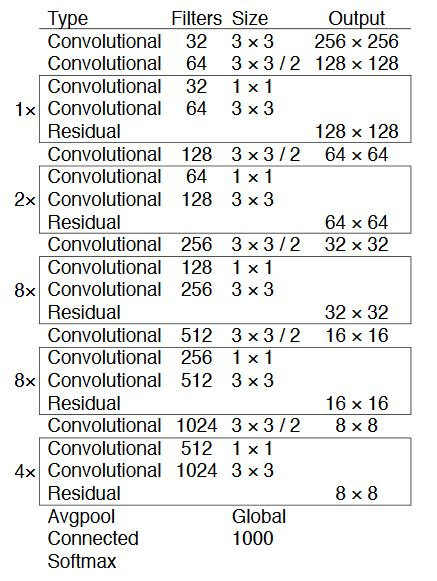
\includegraphics[scale=0.8]{images/yolov3_architecture.jpg}}
  	\caption{Kiến trúc mạng Darknet-53.}
  	\label{fig:bounding_box_prediction}
\end{figure}
Kiến trúc này cho khả năng nhận diện tốt hơn Darknet-19 và hiệu năng cao hơn ResNet-101 hoặc ResNet-152 bảng \ref{table:darknet-53_performance}.
\begin{center}

  \begin{tabular} {l l l l l l}
  \toprule
  \it Backbone & \it Top-1 & \it Top-5 & \it Bn Ops & \it BFLOP/s & \it FPS \\
  \midrule

  Darknet-19 & 74.1 & 91.8 & 7.29 & 1246 & \textbf{171} \\
  ResNet-101 & 77.1 & 93.7 & 19.7 & 1039 & 53 \\
  ResNet-152 & \textbf{77.6} & \textbf{93.8} & 29.4 & 1090 & 37 \\
  Darknet-53 & 77.2 & \textbf{93.8} & 18.7 & 1457 & 78 \\
          
  \bottomrule
  \end{tabular}

\captionof{table}{So sánh hiệu năng của Darknet-53 với các mạng khác. Accuracy, Bn Ops - billions of oper-ations, BFLOP/s - billion floating point operations per second, và FPS - frames per second.
\label{table:darknet-53_performance}}
\end{center}